\documentclass[aspectratio=43, 11pt]{beamer}

\usepackage{fontspec}
\usepackage[spanish, bidi=basic, provide=*]{babel}
\babelprovide[import, onchar=ids fonts]{english}
\babelfont{rm}{Noto Sans}
\babelfont{sf}{Noto Sans}
\usefonttheme{professionalfonts}

\usepackage{amsmath, amssymb}
\usepackage{booktabs}
\usepackage{tikz}
\usetikzlibrary{arrows.meta, babel}

% Paleta sobria y de alto contraste para proyeccion
\definecolor{accentblue}{RGB}{24, 78, 119}
\definecolor{softblue}{RGB}{234, 242, 250}
\definecolor{accentred}{RGB}{192, 57, 43}
\definecolor{accentteal}{RGB}{18, 137, 122}
\definecolor{accentorange}{RGB}{211, 84, 0}
\definecolor{mutedgray}{RGB}{90, 100, 110}

\setbeamertemplate{navigation symbols}{}
\setbeamercolor{structure}{fg=accentblue}
\setbeamercolor{frametitle}{fg=white, bg=accentblue}
\setbeamercolor{title}{fg=accentblue}
\setbeamercolor{block title}{fg=white, bg=accentblue}
\setbeamercolor{block body}{fg=black, bg=softblue}
\setbeamercolor{alerted text}{fg=accentred}
\setbeamertemplate{itemize item}{\color{accentblue}\textbullet}
\setbeamertemplate{itemize subitem}{\color{mutedgray}--}

\setbeamertemplate{footline}{
  \leavevmode%
  \hbox{%
    \begin{beamercolorbox}[wd=.82\paperwidth,ht=2.4ex,dp=1.1ex,leftskip=1.2em]{author in head/foot}%
      \color{mutedgray}\scriptsize Electromagnetismo --- Corriente de desplazamiento
    \end{beamercolorbox}%
    \begin{beamercolorbox}[wd=.18\paperwidth,ht=2.4ex,dp=1.1ex,rightskip=1.2em]{date in head/foot}%
      \hfill\color{accentblue}\scriptsize\bfseries \insertframenumber{} / \inserttotalframenumber
    \end{beamercolorbox}%
  }%
}

\begin{document}

% =====================================================================
% TRANSPARENCIA 1: FEYNMAN, AMPERE-MAXWELL Y CONTINUIDAD DEL FLUJO
% =====================================================================
\begin{frame}{1. Ley de Ampère-Maxwell: independencia de la superficie ($r > R$)}
  \vspace{-0.2cm}
  \begin{equation*}
    \oint_{\Gamma} \mathbf{B}\cdot d\mathbf{l}
    = \mu_0 \left( I_{\mathrm{cond}} + I_d \right)
    = \mu_0 \iint_{S} \left( \mathbf{J} + \varepsilon_0 \frac{\partial \mathbf{E}}{\partial t} \right)\cdot d\mathbf{S}
  \end{equation*}

  \vspace{0.05cm}
      \centering
      \begin{tikzpicture}[scale=0.95, every node/.style={font=\scriptsize}]
        % Cables superior e inferior
        \fill[mutedgray!45, draw=mutedgray] (-0.055, 0.45) rectangle (0.055, 2.25);
        \fill[mutedgray!45, draw=mutedgray] (-0.055, -1.25) rectangle (0.055, -0.45);

        % Placas del condensador (radio R = 1.1)
        \fill[accentblue!25, draw=accentblue, thick] (-1.10, 0.34) rectangle (1.10, 0.45);
        \fill[accentblue!25, draw=accentblue, thick] (-1.10, -0.45) rectangle (1.10, -0.34);

        % Cargas + y - en las placas
        \foreach \x in {-0.85, -0.45, 0.45, 0.85} {
          \node[accentblue, scale=0.75] at (\x, 0.56) {$+$};
          \node[accentblue, scale=0.75] at (\x, -0.57) {$-$};
        }

        % Flechas de corriente I (hacia abajo)
        \draw[-{Stealth[length=2.1mm]}, accentorange, very thick] (0.24, 2.18) -- (0.24, 1.68);
        \node[accentorange, right] at (0.24, 1.93) {\bfseries $I$};
        \draw[-{Stealth[length=2.1mm]}, accentorange, very thick] (0.24, -0.62) -- (0.24, -1.12);
        \node[accentorange, right] at (0.24, -0.87) {\bfseries $I$};

        % Campo electrico E entre placas
        \foreach \x in {-0.85, -0.51, -0.17, 0.17, 0.51, 0.85} {
          \draw[-{Stealth[length=1.4mm]}, accentred, semithick] (\x, 0.31) -- (\x, -0.31);
        }
        \node[accentred, right] at (1.12, -0.18) {$\mathbf{E}$};

        % Superficie S1 y lazo Gamma1 (r = 2.15 > R)
        \draw[accentorange, thick, dashed] (-2.15, 1.48) -- (2.15, 1.48);
        \node[accentorange, above] at (1.30, 1.48) {$S_1$};
        \fill[accentorange] (-2.15, 1.48) circle (1.8pt);
        \fill[accentorange] (2.15, 1.48) circle (1.8pt);
        \node[accentorange, above left] at (-2.10, 1.48) {$\Gamma_1$};

        % Cota de radio r > R
        \draw[{Stealth[length=1.6mm]}-{Stealth[length=1.6mm]}, mutedgray, thin] (0.05, 1.98) -- (2.15, 1.98);
        \node[mutedgray, above] at (1.10, 1.96) {$r > R$};

        % Superficie tipo globo S'1 (esquiva la placa superior y pasa por el hueco)
        \draw[accentteal, very thick, dashed]
          (-2.15, 1.48) .. controls (-1.92, 0.08) and (-1.38, 0.0) .. (0.0, 0.0)
          .. controls (1.38, 0.0) and (1.92, 0.08) .. (2.15, 1.48);
        \node[accentteal, right] at (1.72, 0.68) {\bfseries $S'_1$};

        % Superficie plana S2 y lazo Gamma2 en el plano medio
        \draw[mutedgray, thick, dotted] (-2.15, 0.0) -- (2.15, 0.0);
        \fill[mutedgray] (-2.15, 0.0) circle (1.8pt);
        \fill[mutedgray] (2.15, 0.0) circle (1.8pt);
        \node[mutedgray, above left] at (-2.10, 0.02) {$\Gamma_2$};
        \node[mutedgray, above right] at (1.68, 0.02) {$S_2$};

        % Sentido de B (I hacia abajo: entra a la izquierda, sale a la derecha)
        \node[accentblue, below] at (-2.15, -0.08) {$\otimes\,\mathbf{B}$};
        \node[accentblue, below] at (2.15, -0.08) {$\odot\,\mathbf{B}$};

        % Cota del radio de placa R
        \draw[{Stealth[length=1.5mm]}-{Stealth[length=1.5mm]}, accentblue, thin] (0.0, -0.82) -- (-1.10, -0.82);
        \node[accentblue, below] at (-0.55, -0.82) {$R$};
      \end{tikzpicture}
\end{frame}

\begin{frame}{1. Independencia de la superficie ($r > R$)}
      \textbf{\color{accentblue}Superficies con la misma boca $\Gamma$ ($r > R$):}
      \begin{itemize}
        \item \textbf{Plano en el cable ($S_1$):} corta el conductor.
        \[
          I_{\mathrm{cond}} = I, \qquad I_d = 0
        \]
        \item \textbf{Globo ($S'_1$) o plano medio ($S_2$):} esquiva el cable y captura todo el flujo $\Phi_E = Q/\varepsilon_0$.
        \[
          I_{\mathrm{cond}} = 0, \qquad I_d = \varepsilon_0 \frac{d\Phi_E}{dt} = \frac{dQ}{dt} = I
        \]
      \end{itemize}
\end{frame}

\begin{frame}{1. Superficie que atraviesa la placa}
      \begin{itemize}
        \item \textbf{Al cruzar la placa superior en $\rho_c \in [0, R]$:}
        \[
          I_{\mathrm{cond}}(\rho_c) + I_d(\rho_c)
          = I\!\left(1 - \frac{\rho_c^2}{R^2}\right) + I\,\frac{\rho_c^2}{R^2} = I
        \]
      \end{itemize}
  \vspace{0.15cm}
  \begin{block}{Idea clave (solenoidalidad de la corriente total)}
    Como $\nabla \cdot \left(\mathbf{J} + \varepsilon_0 \frac{\partial \mathbf{E}}{\partial t}\right) = 0$, la corriente total de Maxwell es continua y el campo magnético sobre $\Gamma$ vale siempre $B(r) = \dfrac{\mu_0 I}{2\pi r}$, sin depender de la superficie elegida.
  \end{block}
\end{frame}

% =====================================================================
% TRANSPARENCIA 2: MODELO IDEAL VS. CALCULO NUMERICO REAL
% =====================================================================
\begin{frame}{2. Modelo ideal frente al cálculo numérico}
      \centering
      \IfFileExists{perfil_radial_baja_frecuencia_v2.png}{%
        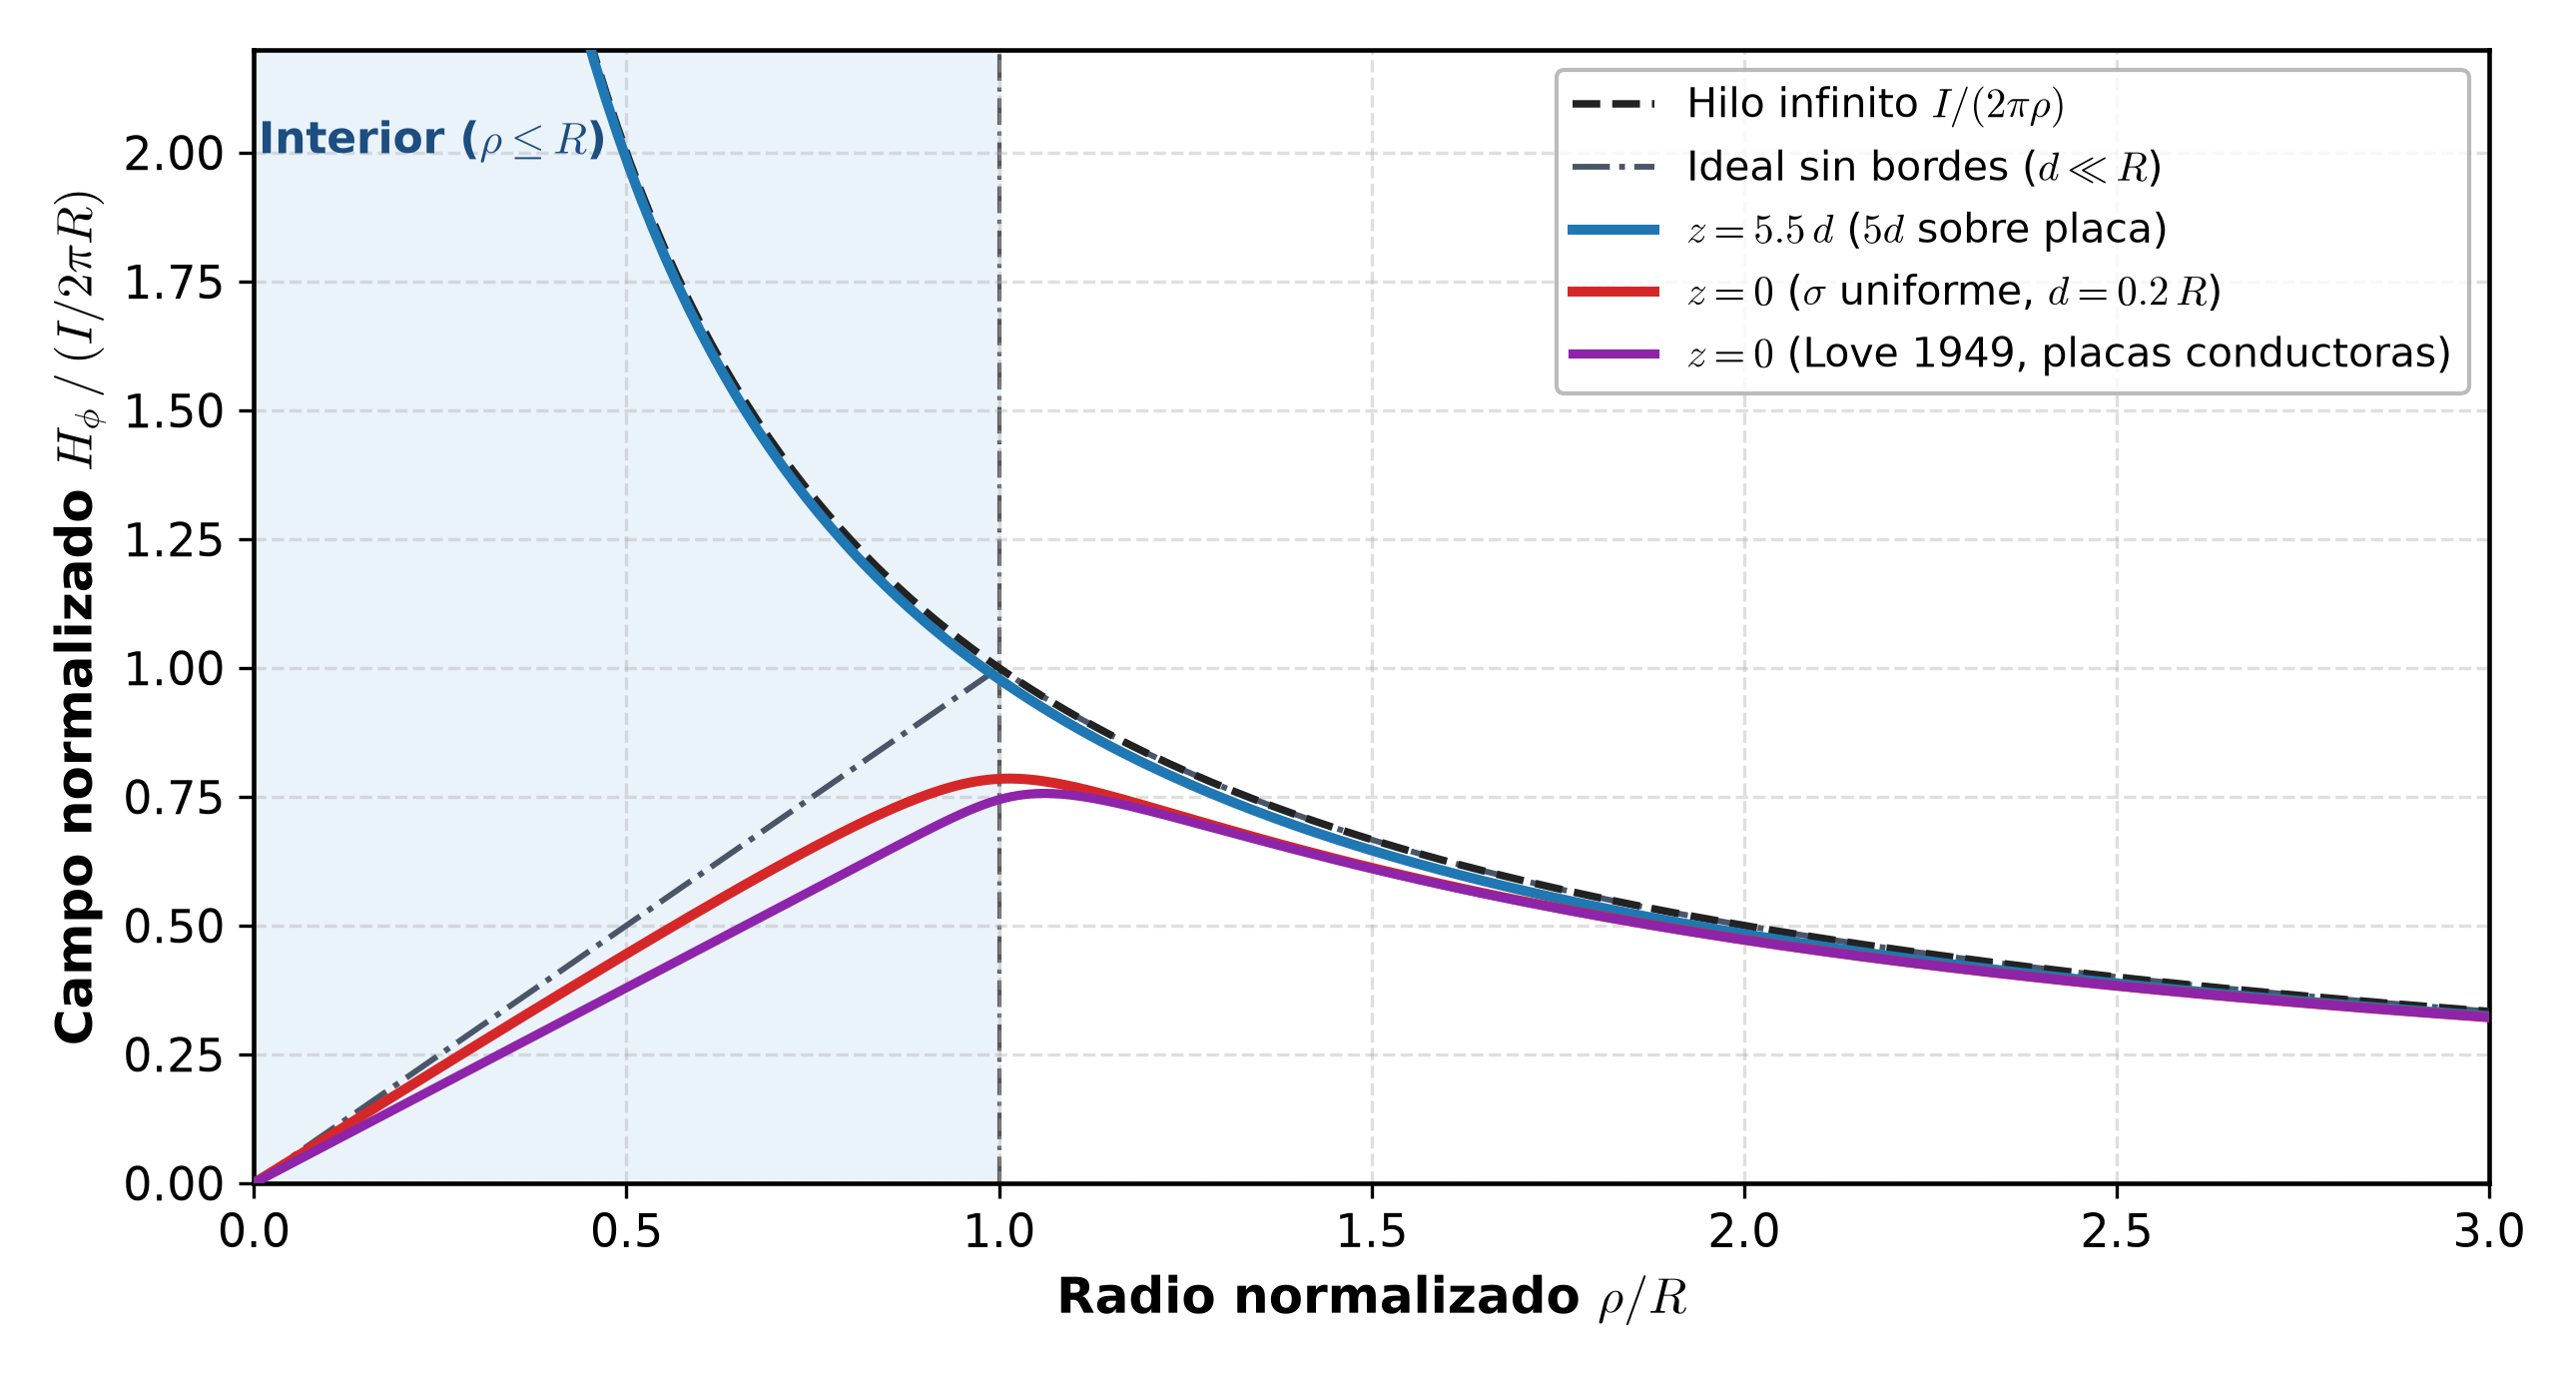
\includegraphics[width=\textwidth,height=0.65\textheight,keepaspectratio]{perfil_radial_baja_frecuencia_v2.png}%
      }{%
        \framebox{\parbox{0.92\textwidth}{\centering\vspace{1.8cm}\texttt{perfil\_radial\_baja\_frecuencia\_v2.png}\\[0.2cm]{\scriptsize\color{mutedgray}(Se insertará automáticamente al compilar con el PNG en la misma carpeta)}\vspace{1.8cm}}}%
      }
      \vspace{0.1cm}
      {\scriptsize\color{mutedgray} Perfil radial normalizado $H_\phi / (I / 2\pi R)$ para $d = 0{,}2\,R$ en régimen cuasiestático ($kR \ll 1$).}
\end{frame}

\begin{frame}{2. ¿Cuadra el modelo ideal?}
      \textbf{\color{accentblue}¿Cuadra el modelo ideal?}
      \vspace{0.15cm}
      \begin{itemize}
        \item \textbf{Exterior ($\rho \gtrsim 1{,}5\,R$) y sobre el cable ($z = 5{,}5\,d$):} el cálculo exacto coincide prácticamente con el hilo infinito $I/(2\pi\rho)$.
        \vspace{0.15cm}
        \item \textbf{Interior ($\rho \le R$, $z = 0$):} los efectos de borde ($d = 0{,}2\,R$) suavizan el pico en $\rho = R$ ($0{,}78\,H_0$ con $\sigma$ uniforme; $0{,}74\,H_0$ con Love 1949), pero conservan el perfil lineal.
        \vspace{0.15cm}
        \item \textbf{Conclusión:} el modelo ideal ($d \ll R$) reproduce \alert{bastante bien} la realidad y valida el argumento de Feynman con $r > R$.
      \end{itemize}
\end{frame}

% =====================================================================
% TRANSPARENCIA 3: CONEXION CON TEORIA DE CIRCUITOS
% =====================================================================
\begin{frame}{3. Conexión con la Teoría de Circuitos}
      \textbf{\color{accentblue}1. Por qué «pasa» corriente por un condensador}
      \vspace{0.15cm}
      \begin{itemize}
        \item Entre las placas no viajan cargas ($I_{\mathrm{cond}} = 0$), pero el flujo eléctrico variable mantiene la continuidad:
        \[
          I_{\mathrm{cable}} = I_{\mathrm{cond}} \;\;=\;\; I_d = \varepsilon_0 \frac{d\Phi_E}{dt}
        \]
        \item Al cerrarse la corriente total $\mathbf{J} + \varepsilon_0 \partial_t\mathbf{E}$ sin fuentes ni sumideros, \textbf{la Ley de Kirchhoff de Corrientes (LKC)} sigue cumpliéndose en cualquier nodo o corte del circuito.
      \end{itemize}
\end{frame}

\begin{frame}{3. De Maxwell a la ecuación $I = C\,dV/dt$}
      \textbf{\color{accentblue}2. De Maxwell a la ecuación $I = C\,\dfrac{dV}{dt}$}
      \vspace{0.15cm}
      \begin{itemize}
        \item En el modelo ideal ($d \ll R$), $E = V/d$ y $\Phi_E = E A = \dfrac{A}{d}\,V$:
        \[
          I = I_d = \varepsilon_0 \frac{d}{dt}\!\left(\frac{A}{d}\,V\right) = \underbrace{\left(\varepsilon_0 \frac{A}{d}\right)}_{C} \frac{dV}{dt}
        \]
        \item Con efectos de borde reales (Love 1949), la estructura $I = C\,\frac{dV}{dt}$ \textbf{no cambia}: solo se corrige el valor efectivo de $C$ ($C/C_{\mathrm{ideal}} \approx 1{,}32$ para $d = 0{,}2\,R$).
      \end{itemize}
\end{frame}

\begin{frame}{3. Frontera de la Teoría de Circuitos}
  \begin{block}{Frontera de la Teoría de Circuitos (parámetros concentrados)}
    La descripción circuital $I = C\,\frac{dV}{dt}$ es exacta mientras $kR = \frac{\omega R}{c} \ll 1$ (régimen cuasiestático). A alta frecuencia ($kR \sim 1$), la inducción de Faraday curva $E_z(\rho) \propto J_0(k\rho)$ y $B_\phi(\rho) \propto J_1(k\rho)$: el condensador deja de ser un elemento concentrado y se comporta como una cavidad resonante.
  \end{block}
\end{frame}

\end{document}